\documentclass[12pt,a4paper,titlepage]{report}
\usepackage[utf8]{inputenc}
\usepackage[francais]{babel}
\usepackage{amsmath}
\usepackage{amsfonts}
\usepackage{amssymb}
\usepackage{graphicx}
\usepackage{url}
\usepackage{hyperref}
\usepackage[hyphenbreaks]{breakurl}
\urlstyle{same}
\hypersetup{ %
colorlinks=false %
,hidelinks %
}


% Police Times
\usepackage{times}

% Mise en forme des tableaux
\usepackage{longtable}
\usepackage{array}
\usepackage{footnote}

% Definition de l'affichage du code
\usepackage{listingsutf8}
\lstset{basicstyle=\footnotesize\ttfamily
%,frame=single
,showstringspaces=false
,tabsize=3
 ,escapeinside={\%*}{*)}
,breaklines=true
,inputencoding=utf8
}
%,extendedchars=false
%,escapeinside=~
% ,inputencoding=latin1
%inputencoding=utf8/latin1
%,backgroundcolor=\color{lightgray}
%,numbers=left
\author{Eric Quinton}
\title{Collec : description des services web}
\date{\today -- v0.1}

%Supprime les veuves et orphelines
\widowpenalty=10000
\clubpenalty=10000
\raggedbottom 
\begin{document}
\maketitle
\chapter{Besoins nécessitant l'utilisation de services web}

\section{Définitions}

\begin{description}
\item[uid:] identifiant unique numérique au sein d'une base de données d'un échan\-tillon ;
\item[guid:] identifiant de type UUID\footnote{Les codes de type GUID ou UUID sont générés à partir de fonctions aléatoires ou cryptographiques, et garantissent qu'ils sont uniques quelle que soit la base de données qui les ont générés. Ainsi, il n'est pas possible d'obtenir deux codes identiques pour deux échantillons différents, ce qui permet de les identifier de manière sûre, comme pourrait le faire l'ADN pour des êtres humains.}, qui garantit de manière certaine l'identification d'un échantillon ;
\item [identifier :] identifiant \og métier \fg{} d'un échantillon;
\item [données \og métier \fg{} :] données permettant de caractériser un échantillon selon les critères nécessaires à son exploitation : contexte spécifique d'acquisition, taxon, données physico-chimiques ou biologiques, etc.
\item [instance, serveur, base de données, application :] implémentation d'une solution de gestion d'échantillons capable soit de fournir des services web, soit d'interroger des services web pour récupérer des informations.
\end{description}
\section{Présentation}
Collec est un logiciel de gestion de collections d'échantillons, dont l'objectif principal consiste à permettre de retrouver rapidement un échantillon stocké ou de récupérer les informations générales le concernant.

Écrit en PHP, les données sont stockées dans une base de données PostgreSQL. Le code de l'application est disponible à l'adresse \url{https://gitlab.com/Irstea/collec}. Il est disponible sous licence AGPL.

Le logiciel est bâti sur un modèle MVC, tous les accès étant gérés par l'appel à des modules déclarés dans un fichier spécifique. Il ne gère pas initialement les URL conviviales (implémenté à partir de la version 1.1).

La gestion matérielle des échantillons de laboratoire (ou d'expérimentations scientifiques) est une fonctionnalité largement demandée, mais peu couverte jusqu'à présent par les logiciels disponibles, et particulièrement dans le domaine de l'\textit{Open Source}. Collec, dont la première version remonte à l'automne 2016, fait l'objet d'un réel intérêt de la part de la communauté scientifique, ses fonctionnalités et sa facilité d'utilisation le rendant attractif.

Toutefois, il n'est pas conçu comme un système global de gestion de données à la fois techniques -- stockage des échantillons -- et de résultats d'analyse par exemple (pas d'informations métiers complexes\footnote{Dans la pratique, à partir de la version 1.1, il est possible de renseigner quelques informations métiers, mais de manière relativement frustre et sans permettre la complexité des actions envisageables avec des bases de données dédiées.}).
Il n'est pas non plus prévu de mettre en place un hébergement centralisé qui permettrait de gérer tous les échantillons de la sphère de recherche.

\textit{A contrario}, cette organisation permet de créer autant d'instances que néces\-saires, notamment pour gérer des saisies en mode décentralisé (bateau partant en campagne de sondage dans les mers du Sud, collecte d'échantillons depuis des zones non couvertes par Internet, par exemple).

Cette souplesse nécessite de prévoir des mécanismes soit d'interrogation de diverses instances, soit de récupération des informations concernant des échantillons provenant d'autres bases de données. 
Pour harmoniser les échanges ou les interrogations, la technologie des services web s'impose, en raison de la normalisation qu'elle apporte.

\subsection{Technique employée}

Les services web sont basés sur des requêtes HTTP, et échangent les données selon des formats définis. Dans la version actuelle des services web, seul le format Json est implémenté pour l'échange des informations.

\subsection{Forme des URL}
Les URL sont conçues, dans le cadre des services web, sous la forme d'URL conviviales, par exemple : \textit{http://collec/sw/v1/sample/4} pour récupérer l'échan\-tillon numéro 4.

\section{Définition des cas d'utilisation couverts par les services web}

SCHEMA

\subsection{Recherche d'échantillons}
La recherche d'échantillons doit pouvoir s'effectuer selon plusieurs critères :
\begin{itemize}
\item l'identifiant interne (\textit{uid});
\item l'identifiant principal ou des identifiants secondaires;
\item une fourchette de dates de création des échantillons;
\item un type d'échantillons;
\item un projet ou sous-collection;
\item une fourchette d'identifiants internes;
\item un code unique de type GUID ou UUID.
\end{itemize}

Elle retourne une liste d'échantillons correspondant aux critères indiqués. Le détail des informations retournées est spécifié dans la section \ref{sampleSearch}.

Pour permettre cette recherche, d'autres services sont nécessaires, notamment pour récupérer la liste des types d'échantillons ou la liste des projets (ou sous-collections).

\subsection{Liste des projets ou sous-collections}
Ce service doit permettre de récupérer la liste des projets ou sous-collections autorisés pour un utilisateur, pour qu'ils puissent servir dans le cadre de la recherche.

\subsection{Liste des types d'échantillons}
Ce service récupère la liste exhaustive des types d'échantillons utilisés dans l'instance distante, pour une utilisation dans le cadre de la recherche.

\subsection{Liste des types d'identifiants secondaires}
Ce service récupère la liste exhaustive des types d'échantillons secondaires, pour une utilisation dans le cadre de la recherche des échantillons.

\subsection{Récupération des données d'un échantillon}
Ce service permet de récupérer l'ensemble des données concernant un échan\-tillon, y compris les données \og métiers \fg{} si l'utilisateur dispose des droits néces\-saires pour les consulter.

Les données récupérées sont suffisamment complètes pour être intégrées dans l'instance \textit{Collec} courante, par exemple pour éviter de les ressaisir suite au prêt d'un échantillon par un laboratoire.

Elles permettent également une visualisation détaillée de l'échantillon consi\-déré, et contiennent, le cas échéant\footnote{si l'utilisateur dispose des droits adéquats et si l'échantillon dispose de ces informations}, les données \og métiers \fg{} associées.

\subsection{Récupération des données d'une liste d'échantillons}

Il s'agit d'une variante du service web précédent. La liste des échantillons à récupérer est fournie dans une collection Json, soit en utilisant l'UID, soit en utilisant le GUID.

\section{Contraintes liées à la sécurité}

Les instances Collec sont prévues pour donner un accès en lecture à toutes les données des échantillons disponibles, dès lors que l'utilisateur s'est identifié. Cela permet ainsi de connaître, par exemple, le produit utilisé pour la conservation ou d'autres informations nécessaires pour la gestion quotidienne des collections.

Toutefois, les données \og métiers \fg ne sont accessibles qu'aux personnes habilitées à les consulter. Dans la pratique, dans Collec, les échantillons sont associés à un projet, et seuls les utilisateurs rattachés à celui-ci peuvent prendre connaissance de ces informations.
Cela impose une gestion particulière des accès lors de l'interrogation par l'intermédiaire des services web, qui sera décrite dans le chapitre \ref{habilitation}.

Le protocole d'identification des utilisateurs dans l'instance distante est basé sur le protocole Oauth v2.



\chapter{Gestion des habilitations -- principes retenus pour le logiciel Collec}
\label{oauth}

Le mécanisme d'identification prévu pour les services web s'appuie en grande partie sur le protocole OAuth v2, au moins dans ses principes. Ce n'est pas le protocole qui est effectivement implémenté (OAuth est prévu pour que l'utilisateur définisse les droits d'accès de l'application cliente), mais les principes d'identification retenus s'en inspirent.

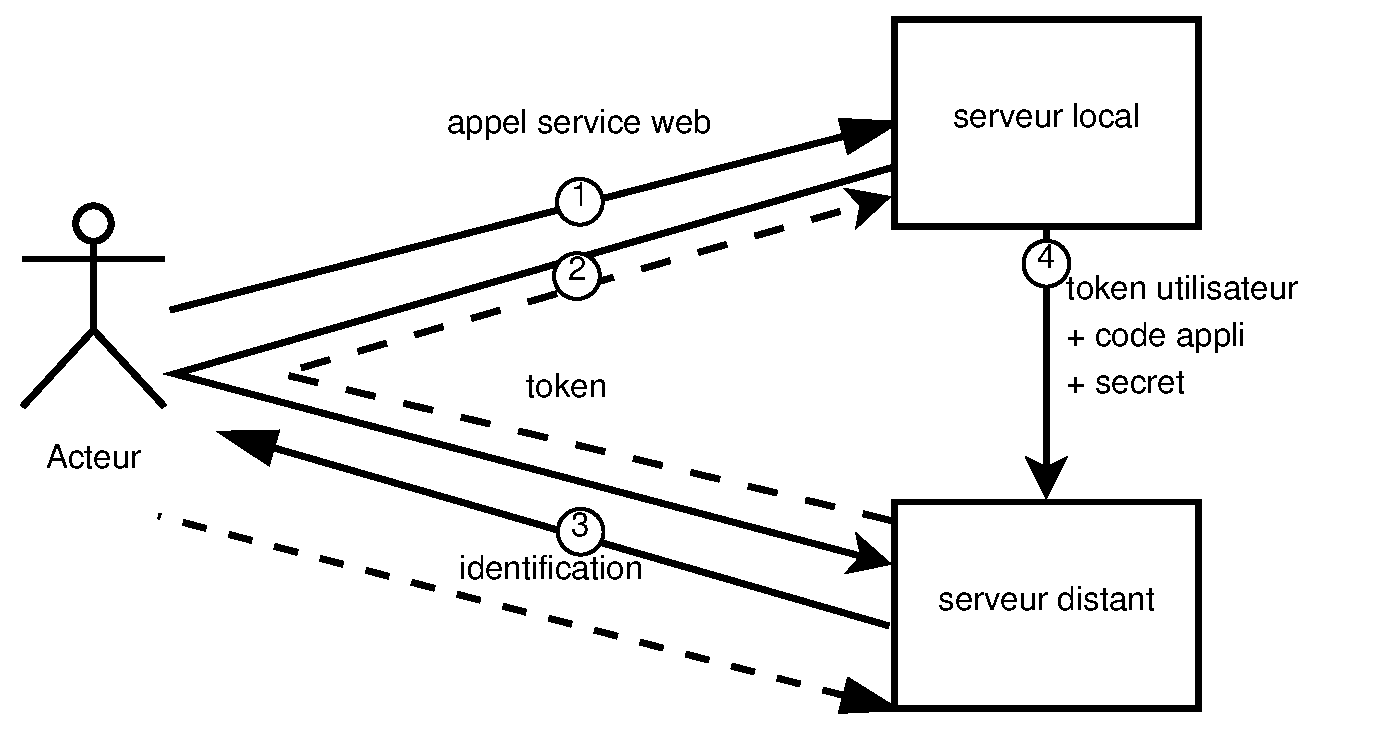
\includegraphics[width=\linewidth]{images/appel_sw_identification}

Pour accéder à des informations distantes, le dialogue entre les deux serveurs nécessite plusieurs phases :
\begin{enumerate}
\item l'utilisateur veut déclencher l'appel à un service web distant ;
\item aucun jeton n'a été récupéré par le serveur local : l'utilisateur est redirigé vers le serveur distant pour obtenir un jeton d'identification;
\item le serveur distant ne connaît pas l'utilisateur : il lui demande de s'identifier en utilisant la procédure adéquate (\textit{login/mot de passe} dans la plupart des cas);
\\une fois identifié, le serveur distant renvoie le navigateur de l'utilisateur vers le serveur local, en fournissant un jeton chiffré;
\item l'appel au service web peut maintenant être déclenché, en fournissant:
\begin{itemize}
\item le jeton de l'utilisateur;
\item le code de l'application locale;
\item le secret partagé entre l'application distante et l'application locale.
\end{itemize}
\end{enumerate}


\section{Opérations préalables à l'interrogation d'une \\base de données distante}
\subsection{Identification réciproque des applications}

Les applications clientes doivent se faire identifier par les applications distantes avant tout échange.

Cette étape est manuelle : l'administrateur de l'application distante crée un enregistrement dans la table \textit{instance}, dont le détail est décrit dans la section \ref{table_instance}.

Le code d'identification, ainsi que le secret associé, est envoyé par mail (de manière automatique ou semi-automatique de préférence) par l'administrateur de la base distante (\textit{cf.} section \ref{dist_record}).

Ces informations sont stockées dans la table \textit{instance} locale, en indiquant en outre les adresses des différents services web disponibles pour le serveur distant.

\subsection{Identification des utilisateurs}
Les utilisateurs qui peuvent utiliser les services web distants sont enregistrés dans le serveur distant et disposent d'un code d'identification. Une fois connectés, ils doivent hériter du droit \textit{consultsw}, indispensable pour accéder aux services web.

Pour qu'ils puissent récupérer les données \og métier \fg{}, les utilisateurs doivent également être rattachés à un projet. Dans la pratique, dans la gestion des groupes de logins, on trouvera l'arborescence suivante (par exemple):
\begin{center}

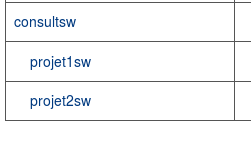
\includegraphics[width=5cm]{images/arborescence_groupes_sw}

\end{center}

Les utilisateurs distants sont associés aux groupes \textit{projet1sw} ou \textit{projet2sw}, et ces groupes sont associés aux projets (ou sous-collections) adéquats pour leur donner les droits d'accès en lecture.

\chapter{Description des services web}
\section{Remarques générales}
\subsection{Format des données transmises ou reçues}

\subsection{Codes d'erreur}


\section{Recherche des échantillons}
\label{sampleSearch}
\subsection{Variables de recherche}
Les variables peuvent être indiquées soit directement dans la requête GET, soit dans le champ \textit{jsonval}, encodé en base 64.

% \usepackage{array} is required
\begin{longtable}{|c|c|>{\raggedright\arraybackslash}p{8cm}|}
\hline 
Code & Type & Description \\ 
\hline \endhead
uid & integer & Identifiant unique de l'échantillon dans l'instance distante \\ 
\hline 
ident & varchar & identifiant \og métier\fg{} principal \\
\hline
guid & UUID & identifiant unique quel que soit la base de données \\
\hline
uidstart & integer & uid inférieur pour une recherche sur une fourchette d'identifiants \\
\hline
uidend & integer & uid supérieur pour une recherche sur une fourchette d'identifiants \\
\hline
datestart & yyyy-mm-dd & date de début pour une recherche sur une fourchette de dates \\
\hline
dateend & yyyy-mm-dd & date de fin pour une recherche sur une fourchette de dates \\
\hline
projectid & integer & identifiant du projet ou de la sous-collection (code issu du résultat du service web \ref{projectList}) \\
\hline
sampletypeid & integer & identifiant du type d'échantillon (code issu du résultat du service web \ref{sampleTypeList}) \\
\hline
idtype & integer & type d'identifiant (code issu du résultat du service web \ref{idtype})\\
\hline
idval & varchar & identifiant recherché selon le type spécifié dans \textit{idtype}\\
\hline
\end{longtable} 

Exemple de fichier : 
\begin{lstlisting}
{"uidstart": 25,
"uidend": 50,
"datestart": "2017-01-01",
"dateend": "2017-06-30",
"idtype": 2,
"idval": "AB01"
}
\end{lstlisting}

\subsection{Données en retour}
Collection Json avec, pour chacun, les informations suivantes :
\begin{longtable}{|c|c|>{\raggedright\arraybackslash}p{6cm}|}
\hline 
Code & Type & Description \\ 
\hline \endhead
uid & integer & Identifiant dans l'instance \\
\hline
identifier & varchar & identifiant principal \og métier\fg{} \\
\hline
guid & uuid & code d'identification global \\
\hline
ids & collection & liste de tous les identifiants secondaires, selon la forme idtype: idval \\
\hline
project & varchar & nom du projet ou de la sous-collection correspondante \\
\hline
createdate & yyyy-mm-dd hh:mm:ss & date de création de l'échantillon dans la base de données d'origine \\
\hline
collectdate & yyyy-mm-dd hh:mm:ss & date de collecte ou de génération de l'échantillon\\
\hline
DATAMETIER & objet json & données \og métier\fg{} rattachées à l'échantillon \\
\hline
sampleparent & objet json & json de même structure que ce tableau comprenant les informations du parent (imbrication des différents parents le cas échéant)\\
\hline
storageproduct & varchar & produit de stockage utilisé \\
\hline
clp & varchar & risques associés aux produit de stockage \\
\hline
subsampletype & varchar & type de sous-échantillonnage \\
\hline
subsampleunit & varchar & unité de sous-échantillonnage \\
\hline
subsampleqty & double & quantité de sous-échantillons présents initialement \\
\hline


\end{longtable}

\section{Lecture d'un échantillon}

La requête, de type GET, contient soit en quatrième valeur, l'UID de l'échantillon à lire, soit la variable \textit{jsonget=}, dont la valeur, encodée en base 64, permet de spécifier le type d'identifiant utilisé :
\begin{longtable}{|c|>{\raggedright\arraybackslash}p{6cm}|}
\hline 
Code & Description \\ 
\hline
Clé & Nom de la variable utilisée \\
\hline
valeur associée & Valeur correspondante\\
\endhead

\end{longtable}

Les valeurs utilisables dans les champs sont les suivants :
\begin{longtable}{|c|c|>{\raggedright\arraybackslash}p{6cm}|}
\hline 
id & Format attendu dans val & Description \\ 
\hline
uid & integer & Clé utilisée dans la base de données \\
\hline
guid & uuid & Identifiant unique global \\
\hline
id & varchar & Identifiant principal de l'échantillon\\
\hline
xxx & varchar & tout code d'identifiant secondaire utilisable dans la base de données distante \\
\hline \endhead

\end{longtable}

Voici un exemple de fichier Json, avant son encodage en base 64:
\begin{lstlisting}
{"uid":25}
\end{lstlisting}

Les données en retour sont celles du service de recherche d'un échantillon.

\section{Lecture d'un jeu d'échantillons}

Il s'agit d'une variante du cas précédent. Le fichier json (encodé en base 64) est organisé pour fournir un identifiant par échantillon retourné. Voici un exemple du fichier :
\begin{lstlisting}
[{"uid":15},{"id":"A1-B2-C3"}]
\end{lstlisting}
Les données en retour sont celles du service de recherche d'un échantillon.

\section{Liste des projets ou sous-collections}
\label{projectList}

La requête est de type GET.
\subsection{Données en entrée}
La requête n'accepte pas de données en entrée.

\subsection{Données en retour}
La requête retourne la liste des projets ou sous-collections autorisées pour l'utilisateur considéré, sous la forme d'une collection Json contenant les informations suivantes :

\begin{longtable}{|c|c|>{\raggedright\arraybackslash}p{6cm}|}
\hline 
Code & Type & Description \\ 
\hline
id & integer & Identifiant interne du projet\\
\hline
val & varchar & Nom du projet\\
\hline
comment & varchar & Description\\
\hline \endhead
\end{longtable}

Exemple :
\begin{lstlisting}
[
{id:1,val:projet1,comment:"Description du projet 1"},
{id:3,val:projet3,comment:"Descripton du projet 3"}
]
\end{lstlisting}



\section{Liste des types d'échantillons}
\label{sampleTypeList}

La requête est de type GET.
\subsection{Données en entrée}
La requête n'accepte pas de données en entrée.

\subsection{Données en retour}
La requête retourne la liste des types d'échantillons, sous la forme d'une collection Json contenant les informations suivantes :

\begin{longtable}{|c|c|>{\raggedright\arraybackslash}p{6cm}|}
\hline 
Code & Type & Description \\ 
\hline
id & integer & Identifiant interne du type d'échantillon\\
\hline
val & varchar & Code du type d'échantillon\\
\hline
comment & varchar & Description\\
\hline \endhead
\end{longtable}

Exemple :
\begin{lstlisting}
[
{id:1,val:projet1,comment:"Description du projet 1"},
{id:3,val:projet3,comment:"Descripton du projet 3"}
]
\end{lstlisting}

\section{Liste des types d'identifiants}
\label{idtype}

La requête est de type GET.
\subsection{Données en entrée}
La requête n'accepte pas de données en entrée.

\subsection{Données en retour}
La requête retourne la liste des types d'identifiants utilisés dans la base de données, sous la forme d'une collection Json contenant les informations suivantes :

\begin{longtable}{|c|c|>{\raggedright\arraybackslash}p{6cm}|}
\hline 
Code & Type & Description \\ 
\hline
id & integer & Identifiant interne du type d'identifiant\\
\hline
val & varchar & Code de l'identifiant\\
\hline
comment & varchar & Description\\
\hline \endhead
\end{longtable}

Exemple :
\begin{lstlisting}
[
{id:1,val:cab,comment:"Code a barres utilise pour l'inventaire"},
{id:2,val:igsn,comment:"Code IGSN pour les carottes de prelevement"}
]
\end{lstlisting}



\chapter{Implémentation technique dans Collec}

Collec est un logiciel de gestion de collections d'échantillons, dont l'objectif principal vise à faciliter la recherche d'un échantillon stocké ou de récupérer les informations générales le concernant.

Écrit en PHP, les données sont stockées dans une base de données PostgreSQL. Le code de l'application est disponible à l'adresse \url{https://gitlab.com/Irstea/collec}. Il est disponible sous licence AGPL.

Le logiciel est bâti sur un modèle MVC, tous les accès étant gérés par l'appel à des modules déclarés dans un fichier spécifique. 

La gestion matérielle des échantillons de laboratoire (ou d'expérimentations scientifiques) est une fonctionnalité largement demandée, mais peu couverte jusqu'à présent par les logiciels disponibles, et particulièrement dans le domaine de l'\textit{Open Source}. Collec, dont la première version remonte à l'automne 2016, fait l'objet d'un réel intérêt de la part de la communauté scientifique, ses fonctionnalités et sa facilité d'utilisation le rendant attractif.

Toutefois, il n'est pas conçu comme un système global de gestion de données à la fois techniques -- stockage des échantillons -- et de résultats d'analyse par exemple (pas d'informations métiers complexes\footnote{Dans la pratique, à partir de la version 1.1, il est possible de renseigner quelques informations métiers, mais de manière relativement frustre et sans permettre la complexité des actions envisageables avec des bases de données dédiées.}).
Il n'est pas non plus prévu de mettre en place un hébergement centralisé qui permettrait de gérer tous les échantillons de la sphère de recherche.

\textit{A contrario}, cette organisation permet de créer autant d'instances que néces\-saires, notamment pour gérer des saisies en mode décentralisé (bateau partant en campagne de sondage dans les mers du Sud, collecte d'échantillons depuis des zones non couvertes par Internet, par exemple).

Cette souplesse nécessite de prévoir des mécanismes soit d'interrogation de diverses instances, soit de récupération des informations concernant des échantillons provenant d'autres bases de données. 

\section{Transformation des URL et appel aux modules}
Les URL conviviales sont transformées en noms de modules, selon le fonctionnement suivant :
\begin{itemize}
\item les trois premiers éléments de l'adresse sont fusionnés;
\item si le quatrième élément est présent, il est stocké dans la variable de requête \textit{\$id}, et :
\begin{itemize}
\item si la requête est de type GET, le module est suffixé par \textit{Display};
\item si la requête est de type POST, le module est suffixé par \textit{Write}\footnote{Dans la version actuelle, l'écriture depuis une instance distante n'est pas implémentée};
\end{itemize}
\item sinon, le module est suffixé par \textit{List}.
\end{itemize}

Les modules doivent être décrits, comme les autres, dans le fichier \textit{param/actions.xml}, et sont exécutés selon le fonctionnement classique de l'application.

\section{Emplacement du code}
Le code spécifique des modules doit être stocké dans le dossier \textit{modules}, en respectant l'arborescence des URL conviviales, par exemple, pour l'adresse \textit{http://collec.local/sw/v1/sample}, dans le sous-dossier \textit{sw/v1}.


\subsection{Données d'identification des instances distantes}
\label{table_instance}

Pour identifier les instances clientes, la table \textit{instance} contient les données suivantes :
\begin{itemize}
\item le nom de l'instance;
\item l'url de l'instance ;
\item le nom d'un contact;
\item son mail;
\item le code attribué en conservant les 8 premiers caractères du calcul d'empreintes sha256 de l'url;
\item le secret, généré de manière cryptographique ;
\item le type d'instance (cliente ou serveur);
\item la date de fin d'autorisation d'accès, par défaut, fixée à 5 ans.
\end{itemize}

Si une instance est à la fois cliente et serveur, deux lignes devront être créées, l'une pour chaque sens de communication. Cela permet de maintenir des secrets différents pour chaque canal.

Pour les instances \og serveurs\fg{}, une table complémentaire permet d'indiquer les URI des services web disponibles :
\begin{itemize}
\item le type du service web;
\item l'URI correspondante;
\item le type d'identification prévu: \textit{OauthV1}, \textit{OauthV2}, pas d'identification.
\end{itemize}

\subsection{Structure des tables correspondantes}



\tableofcontents
\end{document}